% Created by tikzDevice version 0.10.1 on 2018-03-10 15:46:48
% !TEX encoding = UTF-8 Unicode
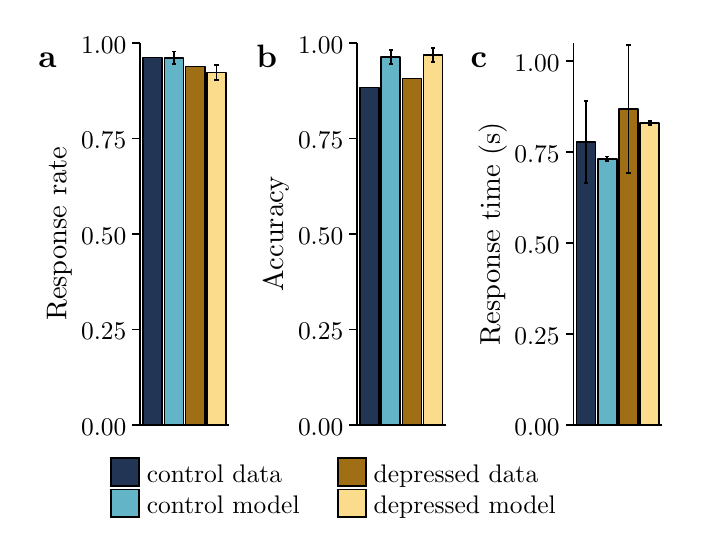
\begin{tikzpicture}[x=1pt,y=1pt]
\definecolor{fillColor}{RGB}{255,255,255}
\path[use as bounding box,fill=fillColor,fill opacity=0.00] (0,0) rectangle (234.88,180.67);
\begin{scope}
\path[clip] (  0.00, 28.91) rectangle ( 78.29,180.67);
\definecolor{drawColor}{RGB}{255,255,255}
\definecolor{fillColor}{RGB}{255,255,255}

\path[draw=drawColor,line width= 0.6pt,line join=round,line cap=round,fill=fillColor] (  0.00, 28.91) rectangle ( 78.29,180.67);
\end{scope}
\begin{scope}
\path[clip] ( 40.61, 37.16) rectangle ( 72.79,175.17);
\definecolor{fillColor}{RGB}{255,255,255}

\path[fill=fillColor] ( 40.61, 37.16) rectangle ( 72.79,175.17);
\definecolor{drawColor}{RGB}{0,0,0}
\definecolor{fillColor}{RGB}{35,53,85}

\path[draw=drawColor,line width= 0.6pt,line join=round,fill=fillColor] ( 41.76, 37.16) rectangle ( 48.65,169.88);
\definecolor{fillColor}{RGB}{100,180,200}

\path[draw=drawColor,line width= 0.6pt,line join=round,fill=fillColor] ( 49.42, 37.16) rectangle ( 56.32,169.74);
\definecolor{fillColor}{RGB}{160,110,20}

\path[draw=drawColor,line width= 0.6pt,line join=round,fill=fillColor] ( 57.08, 37.16) rectangle ( 63.98,166.66);
\definecolor{fillColor}{RGB}{250,220,140}

\path[draw=drawColor,line width= 0.6pt,line join=round,fill=fillColor] ( 64.75, 37.16) rectangle ( 71.64,164.48);

\path[draw=drawColor,line width= 0.6pt,line join=round] ( 52.10,172.03) --
	( 53.64,172.03);

\path[draw=drawColor,line width= 0.6pt,line join=round] ( 52.87,172.03) --
	( 52.87,167.45);

\path[draw=drawColor,line width= 0.6pt,line join=round] ( 52.10,167.45) --
	( 53.64,167.45);

\path[draw=drawColor,line width= 0.6pt,line join=round] ( 67.43,167.29) --
	( 68.96,167.29);

\path[draw=drawColor,line width= 0.6pt,line join=round] ( 68.19,167.29) --
	( 68.19,161.66);

\path[draw=drawColor,line width= 0.6pt,line join=round] ( 67.43,161.66) --
	( 68.96,161.66);
\end{scope}
\begin{scope}
\path[clip] (  0.00,  0.00) rectangle (234.88,180.67);
\definecolor{drawColor}{RGB}{0,0,0}

\path[draw=drawColor,line width= 0.6pt,line join=round] ( 40.61, 37.16) --
	( 40.61,175.17);
\end{scope}
\begin{scope}
\path[clip] (  0.00,  0.00) rectangle (234.88,180.67);
\definecolor{drawColor}{RGB}{0,0,0}

\node[text=drawColor,anchor=base east,inner sep=0pt, outer sep=0pt, scale=  0.92] at ( 35.66, 33.37) {0.00};

\node[text=drawColor,anchor=base east,inner sep=0pt, outer sep=0pt, scale=  0.92] at ( 35.66, 67.87) {0.25};

\node[text=drawColor,anchor=base east,inner sep=0pt, outer sep=0pt, scale=  0.92] at ( 35.66,102.38) {0.50};

\node[text=drawColor,anchor=base east,inner sep=0pt, outer sep=0pt, scale=  0.92] at ( 35.66,136.88) {0.75};

\node[text=drawColor,anchor=base east,inner sep=0pt, outer sep=0pt, scale=  0.92] at ( 35.66,171.39) {1.00};
\end{scope}
\begin{scope}
\path[clip] (  0.00,  0.00) rectangle (234.88,180.67);
\definecolor{drawColor}{RGB}{0,0,0}

\path[draw=drawColor,line width= 0.6pt,line join=round] ( 37.86, 37.16) --
	( 40.61, 37.16);

\path[draw=drawColor,line width= 0.6pt,line join=round] ( 37.86, 71.66) --
	( 40.61, 71.66);

\path[draw=drawColor,line width= 0.6pt,line join=round] ( 37.86,106.17) --
	( 40.61,106.17);

\path[draw=drawColor,line width= 0.6pt,line join=round] ( 37.86,140.67) --
	( 40.61,140.67);

\path[draw=drawColor,line width= 0.6pt,line join=round] ( 37.86,175.17) --
	( 40.61,175.17);
\end{scope}
\begin{scope}
\path[clip] (  0.00,  0.00) rectangle (234.88,180.67);
\definecolor{drawColor}{RGB}{0,0,0}

\path[draw=drawColor,line width= 0.6pt,line join=round] ( 40.61, 37.16) --
	( 72.79, 37.16);
\end{scope}
\begin{scope}
\path[clip] (  0.00,  0.00) rectangle (234.88,180.67);
\definecolor{drawColor}{RGB}{0,0,0}

\node[text=drawColor,rotate= 90.00,anchor=base,inner sep=0pt, outer sep=0pt, scale=  1.03] at ( 14.02,106.17) {Response rate};
\end{scope}
\begin{scope}
\path[clip] (  0.00,  0.00) rectangle (234.88,180.67);
\definecolor{drawColor}{RGB}{0,0,0}

\node[text=drawColor,anchor=base west,inner sep=0pt, outer sep=0pt, scale=  1.17] at (  3.83,166.18) {\bfseries a};
\end{scope}
\begin{scope}
\path[clip] ( 78.29, 28.91) rectangle (156.59,180.67);
\definecolor{drawColor}{RGB}{255,255,255}
\definecolor{fillColor}{RGB}{255,255,255}

\path[draw=drawColor,line width= 0.6pt,line join=round,line cap=round,fill=fillColor] ( 78.29, 28.91) rectangle (156.59,180.67);
\end{scope}
\begin{scope}
\path[clip] (118.99, 37.16) rectangle (151.09,175.17);
\definecolor{fillColor}{RGB}{255,255,255}

\path[fill=fillColor] (118.99, 37.16) rectangle (151.09,175.17);
\definecolor{drawColor}{RGB}{0,0,0}
\definecolor{fillColor}{RGB}{35,53,85}

\path[draw=drawColor,line width= 0.6pt,line join=round,fill=fillColor] (120.13, 37.16) rectangle (127.01,159.07);
\definecolor{fillColor}{RGB}{100,180,200}

\path[draw=drawColor,line width= 0.6pt,line join=round,fill=fillColor] (127.77, 37.16) rectangle (134.65,170.17);
\definecolor{fillColor}{RGB}{160,110,20}

\path[draw=drawColor,line width= 0.6pt,line join=round,fill=fillColor] (135.42, 37.16) rectangle (142.30,162.29);
\definecolor{fillColor}{RGB}{250,220,140}

\path[draw=drawColor,line width= 0.6pt,line join=round,fill=fillColor] (143.06, 37.16) rectangle (149.94,170.79);

\path[draw=drawColor,line width= 0.6pt,line join=round] (130.45,172.69) --
	(131.98,172.69);

\path[draw=drawColor,line width= 0.6pt,line join=round] (131.21,172.69) --
	(131.21,167.64);

\path[draw=drawColor,line width= 0.6pt,line join=round] (130.45,167.64) --
	(131.98,167.64);

\path[draw=drawColor,line width= 0.6pt,line join=round] (145.74,173.32) --
	(147.26,173.32);

\path[draw=drawColor,line width= 0.6pt,line join=round] (146.50,173.32) --
	(146.50,168.25);

\path[draw=drawColor,line width= 0.6pt,line join=round] (145.74,168.25) --
	(147.26,168.25);
\end{scope}
\begin{scope}
\path[clip] (  0.00,  0.00) rectangle (234.88,180.67);
\definecolor{drawColor}{RGB}{0,0,0}

\path[draw=drawColor,line width= 0.6pt,line join=round] (118.99, 37.16) --
	(118.99,175.17);
\end{scope}
\begin{scope}
\path[clip] (  0.00,  0.00) rectangle (234.88,180.67);
\definecolor{drawColor}{RGB}{0,0,0}

\node[text=drawColor,anchor=base east,inner sep=0pt, outer sep=0pt, scale=  0.92] at (114.04, 33.37) {0.00};

\node[text=drawColor,anchor=base east,inner sep=0pt, outer sep=0pt, scale=  0.92] at (114.04, 67.87) {0.25};

\node[text=drawColor,anchor=base east,inner sep=0pt, outer sep=0pt, scale=  0.92] at (114.04,102.38) {0.50};

\node[text=drawColor,anchor=base east,inner sep=0pt, outer sep=0pt, scale=  0.92] at (114.04,136.88) {0.75};

\node[text=drawColor,anchor=base east,inner sep=0pt, outer sep=0pt, scale=  0.92] at (114.04,171.39) {1.00};
\end{scope}
\begin{scope}
\path[clip] (  0.00,  0.00) rectangle (234.88,180.67);
\definecolor{drawColor}{RGB}{0,0,0}

\path[draw=drawColor,line width= 0.6pt,line join=round] (116.24, 37.16) --
	(118.99, 37.16);

\path[draw=drawColor,line width= 0.6pt,line join=round] (116.24, 71.66) --
	(118.99, 71.66);

\path[draw=drawColor,line width= 0.6pt,line join=round] (116.24,106.17) --
	(118.99,106.17);

\path[draw=drawColor,line width= 0.6pt,line join=round] (116.24,140.67) --
	(118.99,140.67);

\path[draw=drawColor,line width= 0.6pt,line join=round] (116.24,175.17) --
	(118.99,175.17);
\end{scope}
\begin{scope}
\path[clip] (  0.00,  0.00) rectangle (234.88,180.67);
\definecolor{drawColor}{RGB}{0,0,0}

\path[draw=drawColor,line width= 0.6pt,line join=round] (118.99, 37.16) --
	(151.09, 37.16);
\end{scope}
\begin{scope}
\path[clip] (  0.00,  0.00) rectangle (234.88,180.67);
\definecolor{drawColor}{RGB}{0,0,0}

\node[text=drawColor,rotate= 90.00,anchor=base,inner sep=0pt, outer sep=0pt, scale=  1.03] at ( 92.31,106.17) {Accuracy};
\end{scope}
\begin{scope}
\path[clip] (  0.00,  0.00) rectangle (234.88,180.67);
\definecolor{drawColor}{RGB}{0,0,0}

\node[text=drawColor,anchor=base west,inner sep=0pt, outer sep=0pt, scale=  1.17] at ( 82.67,166.18) {\bfseries b};
\end{scope}
\begin{scope}
\path[clip] (156.59, 28.91) rectangle (234.88,180.67);
\definecolor{drawColor}{RGB}{255,255,255}
\definecolor{fillColor}{RGB}{255,255,255}

\path[draw=drawColor,line width= 0.6pt,line join=round,line cap=round,fill=fillColor] (156.59, 28.91) rectangle (234.88,180.67);
\end{scope}
\begin{scope}
\path[clip] (197.19, 37.16) rectangle (229.38,175.17);
\definecolor{fillColor}{RGB}{255,255,255}

\path[fill=fillColor] (197.19, 37.16) rectangle (229.38,175.17);
\definecolor{drawColor}{RGB}{0,0,0}
\definecolor{fillColor}{RGB}{35,53,85}

\path[draw=drawColor,line width= 0.6pt,line join=round,fill=fillColor] (198.34, 37.16) rectangle (205.24,139.33);
\definecolor{fillColor}{RGB}{100,180,200}

\path[draw=drawColor,line width= 0.6pt,line join=round,fill=fillColor] (206.01, 37.16) rectangle (212.90,133.24);
\definecolor{fillColor}{RGB}{160,110,20}

\path[draw=drawColor,line width= 0.6pt,line join=round,fill=fillColor] (213.67, 37.16) rectangle (220.57,151.30);
\definecolor{fillColor}{RGB}{250,220,140}

\path[draw=drawColor,line width= 0.6pt,line join=round,fill=fillColor] (221.33, 37.16) rectangle (228.23,146.24);

\path[draw=drawColor,line width= 0.6pt,line join=round] (201.02,154.08) --
	(202.56,154.08);

\path[draw=drawColor,line width= 0.6pt,line join=round] (201.79,154.08) --
	(201.79,124.59);

\path[draw=drawColor,line width= 0.6pt,line join=round] (201.02,124.59) --
	(202.56,124.59);

\path[draw=drawColor,line width= 0.6pt,line join=round] (208.69,134.06) --
	(210.22,134.06);

\path[draw=drawColor,line width= 0.6pt,line join=round] (209.45,134.06) --
	(209.45,132.42);

\path[draw=drawColor,line width= 0.6pt,line join=round] (208.69,132.42) --
	(210.22,132.42);

\path[draw=drawColor,line width= 0.6pt,line join=round] (216.35,174.45) --
	(217.88,174.45);

\path[draw=drawColor,line width= 0.6pt,line join=round] (217.12,174.45) --
	(217.12,128.14);

\path[draw=drawColor,line width= 0.6pt,line join=round] (216.35,128.14) --
	(217.88,128.14);

\path[draw=drawColor,line width= 0.6pt,line join=round] (224.01,147.02) --
	(225.55,147.02);

\path[draw=drawColor,line width= 0.6pt,line join=round] (224.78,147.02) --
	(224.78,145.46);

\path[draw=drawColor,line width= 0.6pt,line join=round] (224.01,145.46) --
	(225.55,145.46);
\end{scope}
\begin{scope}
\path[clip] (  0.00,  0.00) rectangle (234.88,180.67);
\definecolor{drawColor}{RGB}{0,0,0}

\path[draw=drawColor,line width= 0.6pt,line join=round] (197.19, 37.16) --
	(197.19,175.17);
\end{scope}
\begin{scope}
\path[clip] (  0.00,  0.00) rectangle (234.88,180.67);
\definecolor{drawColor}{RGB}{0,0,0}

\node[text=drawColor,anchor=base east,inner sep=0pt, outer sep=0pt, scale=  0.92] at (192.24, 33.37) {0.00};

\node[text=drawColor,anchor=base east,inner sep=0pt, outer sep=0pt, scale=  0.92] at (192.24, 66.23) {0.25};

\node[text=drawColor,anchor=base east,inner sep=0pt, outer sep=0pt, scale=  0.92] at (192.24, 99.09) {0.50};

\node[text=drawColor,anchor=base east,inner sep=0pt, outer sep=0pt, scale=  0.92] at (192.24,131.95) {0.75};

\node[text=drawColor,anchor=base east,inner sep=0pt, outer sep=0pt, scale=  0.92] at (192.24,164.81) {1.00};
\end{scope}
\begin{scope}
\path[clip] (  0.00,  0.00) rectangle (234.88,180.67);
\definecolor{drawColor}{RGB}{0,0,0}

\path[draw=drawColor,line width= 0.6pt,line join=round] (194.44, 37.16) --
	(197.19, 37.16);

\path[draw=drawColor,line width= 0.6pt,line join=round] (194.44, 70.02) --
	(197.19, 70.02);

\path[draw=drawColor,line width= 0.6pt,line join=round] (194.44,102.88) --
	(197.19,102.88);

\path[draw=drawColor,line width= 0.6pt,line join=round] (194.44,135.74) --
	(197.19,135.74);

\path[draw=drawColor,line width= 0.6pt,line join=round] (194.44,168.60) --
	(197.19,168.60);
\end{scope}
\begin{scope}
\path[clip] (  0.00,  0.00) rectangle (234.88,180.67);
\definecolor{drawColor}{RGB}{0,0,0}

\path[draw=drawColor,line width= 0.6pt,line join=round] (197.19, 37.16) --
	(229.38, 37.16);
\end{scope}
\begin{scope}
\path[clip] (  0.00,  0.00) rectangle (234.88,180.67);
\definecolor{drawColor}{RGB}{0,0,0}

\node[text=drawColor,rotate= 90.00,anchor=base,inner sep=0pt, outer sep=0pt, scale=  1.03] at (170.61,106.17) {Response time (s)};
\end{scope}
\begin{scope}
\path[clip] (  0.00,  0.00) rectangle (234.88,180.67);
\definecolor{drawColor}{RGB}{0,0,0}

\node[text=drawColor,anchor=base west,inner sep=0pt, outer sep=0pt, scale=  1.17] at (160.09,166.18) {\bfseries c};
\end{scope}
\begin{scope}
\path[clip] (  0.00,  0.00) rectangle (234.88,180.67);
\definecolor{fillColor}{RGB}{255,255,255}

\path[fill=fillColor] ( 19.47, -2.62) rectangle (215.41, 31.53);
\end{scope}
\begin{scope}
\path[clip] (  0.00,  0.00) rectangle (234.88,180.67);
\definecolor{drawColor}{RGB}{0,0,0}
\definecolor{fillColor}{RGB}{35,53,85}

\path[draw=drawColor,line width= 0.6pt,line cap=round,fill=fillColor] ( 30.21, 15.17) rectangle ( 40.17, 25.12);
\end{scope}
\begin{scope}
\path[clip] (  0.00,  0.00) rectangle (234.88,180.67);
\definecolor{drawColor}{RGB}{0,0,0}
\definecolor{fillColor}{RGB}{100,180,200}

\path[draw=drawColor,line width= 0.6pt,line cap=round,fill=fillColor] ( 30.21,  3.78) rectangle ( 40.17, 13.74);
\end{scope}
\begin{scope}
\path[clip] (  0.00,  0.00) rectangle (234.88,180.67);
\definecolor{drawColor}{RGB}{0,0,0}
\definecolor{fillColor}{RGB}{160,110,20}

\path[draw=drawColor,line width= 0.6pt,line cap=round,fill=fillColor] (112.19, 15.17) rectangle (122.15, 25.12);
\end{scope}
\begin{scope}
\path[clip] (  0.00,  0.00) rectangle (234.88,180.67);
\definecolor{drawColor}{RGB}{0,0,0}
\definecolor{fillColor}{RGB}{250,220,140}

\path[draw=drawColor,line width= 0.6pt,line cap=round,fill=fillColor] (112.19,  3.78) rectangle (122.15, 13.74);
\end{scope}
\begin{scope}
\path[clip] (  0.00,  0.00) rectangle (234.88,180.67);
\definecolor{drawColor}{RGB}{0,0,0}

\node[text=drawColor,anchor=base west,inner sep=0pt, outer sep=0pt, scale=  0.92] at ( 43.04, 16.36) {control data};
\end{scope}
\begin{scope}
\path[clip] (  0.00,  0.00) rectangle (234.88,180.67);
\definecolor{drawColor}{RGB}{0,0,0}

\node[text=drawColor,anchor=base west,inner sep=0pt, outer sep=0pt, scale=  0.92] at ( 43.04,  4.98) {control model};
\end{scope}
\begin{scope}
\path[clip] (  0.00,  0.00) rectangle (234.88,180.67);
\definecolor{drawColor}{RGB}{0,0,0}

\node[text=drawColor,anchor=base west,inner sep=0pt, outer sep=0pt, scale=  0.92] at (125.03, 16.36) {depressed data};
\end{scope}
\begin{scope}
\path[clip] (  0.00,  0.00) rectangle (234.88,180.67);
\definecolor{drawColor}{RGB}{0,0,0}

\node[text=drawColor,anchor=base west,inner sep=0pt, outer sep=0pt, scale=  0.92] at (125.03,  4.98) {depressed model};
\end{scope}
\end{tikzpicture}
